%!TEX root = ../thesis.tex

\section{背景}
近年,人手不足を背景にサービスロボットの需要が高まり,オフィスロボットの開発が活発化している.PAL Robotics社のTIAGo(図\ref{fig:TIAGo})やトヨタ自動車のHSR(図\ref{fig:HSR})など,様々なオフィスロボットが開発されているが,設計データを公開しているロボットが少なく,ユーザによる改良や研究開発への新規参入が困難となっている.また,市販のオフィスロボットは,高度なセンサ構成などのため,高価格である場合が多く,コスト面で大きな負担となる.そのため,研究開発用途に適した,容易に利用・改変可能なオープンプラットフォームなオフィスロボットは依然として不足しているのが現状である.

このような状況に対し,オープンプラットフォームハードウェアの成功事例として,i-Cartシリーズが挙げられる.自律移動ロボットであるi-Cart miniとi-Cart middleは,設計データ,部品リスト,組み立て図を公開しており,誰もが容易に複製・改良できる.i-Cartをベースとした様々なロボットが開発され,自律移動ロボット開発の活性化に大きく貢献している.これは,i-Cartシリーズの登場により,自律移動ロボット開発への参入障壁が大幅に低下したことを示唆している.そのため,オープンプラットフォームオフィスロボットを開発し,研究開発への参入障壁を下げることを目指す.

\begin{figure}[h]
  \centering
  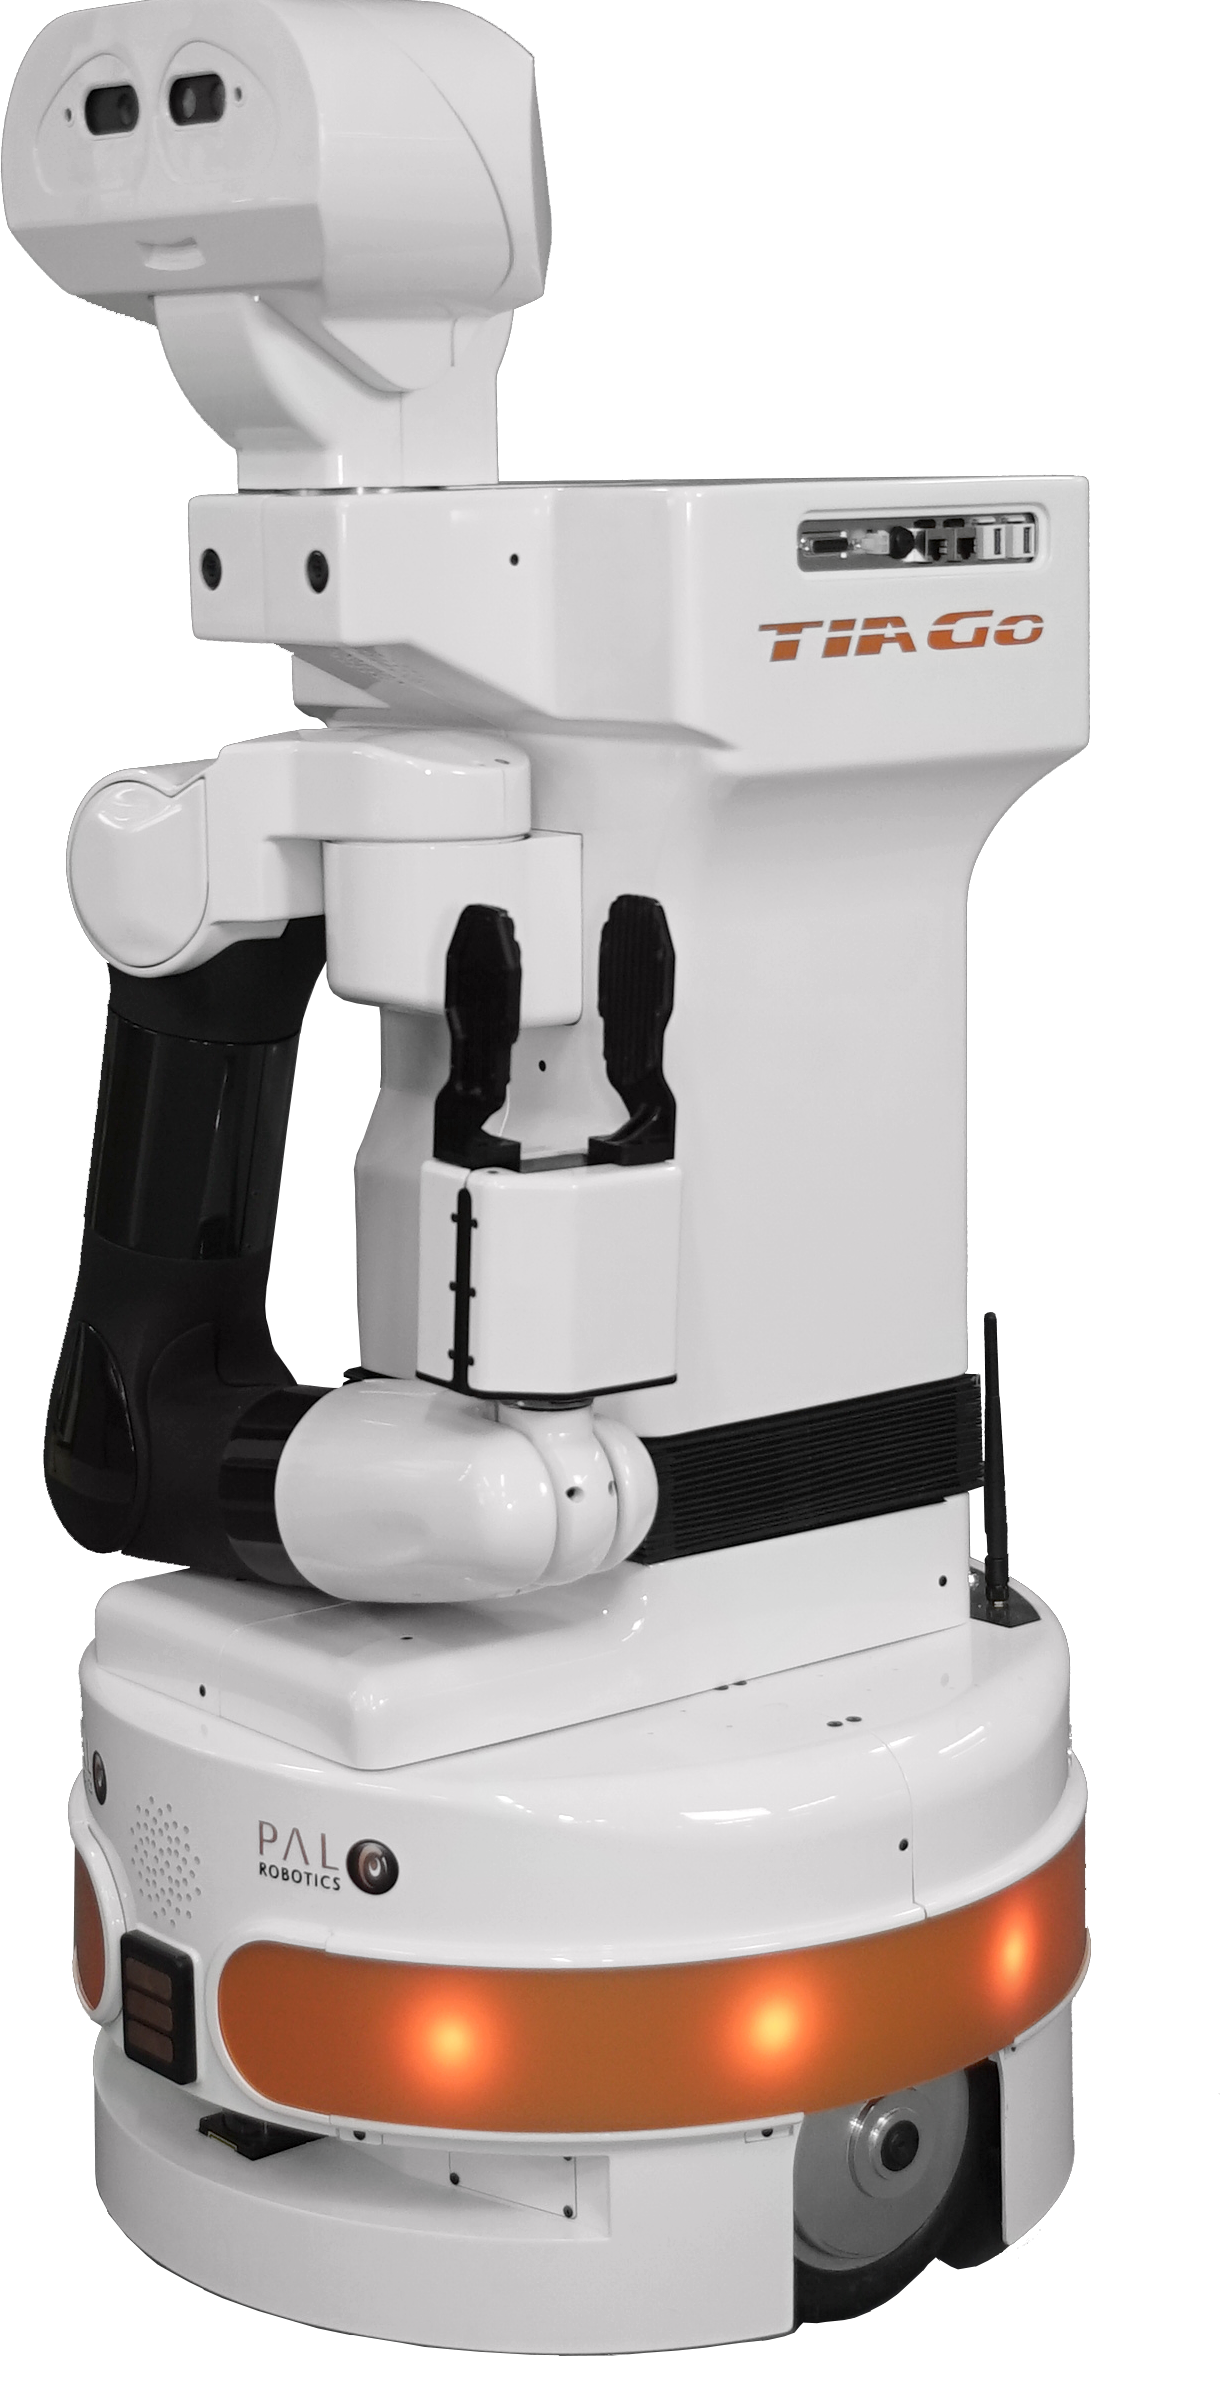
\includegraphics[width=25mm]{images/png/TIAGo.png}
  \caption{TIAGo from PAL-Robotics (source: \cite{TIAGo:online})}
  \label{fig:TIAGo}
\end{figure}
\begin{figure}[h]
  \centering
  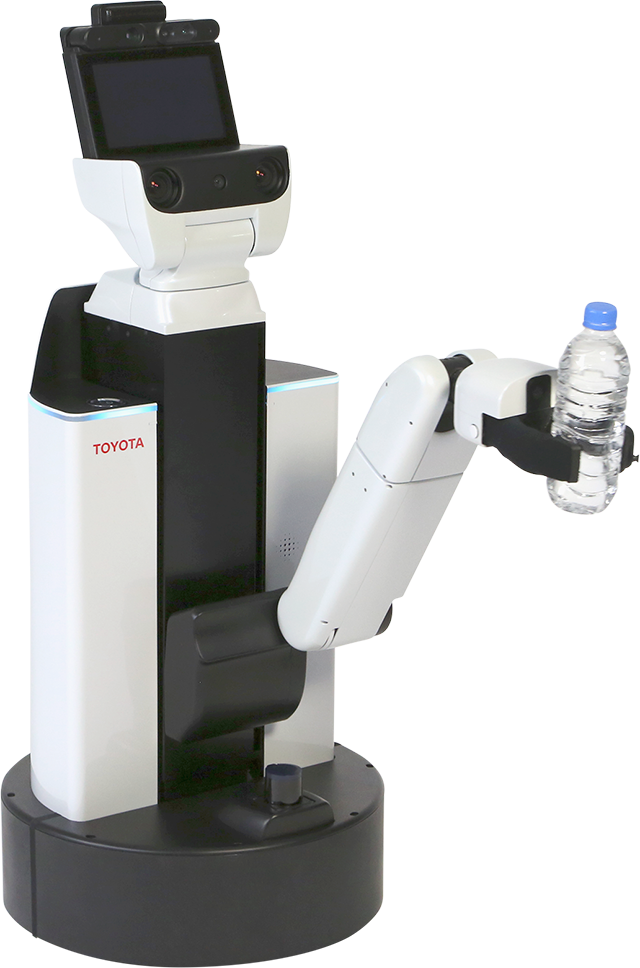
\includegraphics[width=25mm]{images/png/HSR.png}
  \caption{HSR from TOYOTA (source: \cite{HSR:online})}
  \label{fig:HSR}
\end{figure}

\begin{table}[h]
  \centering
  \caption{Comparison of actuators used in existing office robot arms and QDD motors}
  \begin{tabular}{lccc}
  \hline
            & \begin{tabular}[c]{@{}c@{}}Dynamixel \\ MX-106T\end{tabular} & \begin{tabular}[c]{@{}c@{}}KONDO\\ B3M-CS-1170-A\end{tabular} & \begin{tabular}[c]{@{}c@{}}Steadywin\\ GIM8108-8\end{tabular} \\ \hline
  ストールトルク[Nm]   & 8.0                                                          & 7.6                                                           & 22                                                            \\
  無負荷回転数[rpm]    & 41                                                           & 46                                                            & 110                                                           \\
  減速比       & 225 : 1                                                      & 362.88 : 1                                                    & 8 : 1                                                         \\
  重量[g]        & 153                                                          & 105                                                           & 396                                                           \\
  許容ラジアル荷重[N]  & 40                                                           & -                                                             & 900                                                           \\
  許容アキシアル荷重[N] & 20                                                           & -                                                             & 800                                                           \\ \hline
  \end{tabular}
  \label{table:motor}
\end{table}
\clearpage
\newpage